\section{Authenticated Retrieval over Loopback TCP}
\label{sec:layout-transfer}

Separate client/server processes exchange setup and queries over loopback TCP. Online wall time includes routing, query generation, exchange, decoding, proof assembly, and root verification; startup and bootstrap are excluded. Traffic includes application framing but excludes TCP/IP headers. Each method uses five independent process pairs, five warmups, and 100 paired targets with randomized method order. Student's $t$ intervals use process-pair means and four degrees of freedom. WAN behavior is unmeasured.

\subsection{Fuel: an optimal bucket capacity does not reduce traffic}
\label{sec:fuel-layout-transfer}

First-fit, AB, an independently certified capacity-22 witness, and Full-cache share Fuel slots, values, 198 active digests, and root at $h=128$. The witness is separate from AB and bounded recoloring. Each digest uses eight 32-bit SimplePIR chunks with common lattice/noise parameters; clients already know their slot/value pair.

\begin{table*}[t]
\centering\small\setlength{\tabcolsep}{5pt}
\caption{Fuel TCP results under SimplePIR~\cite{simplepir}. AB is ours; the remaining rows are internal controls. Q/A/R denote query/answer/recovery times; E2E has a 95\% $t$ interval over five process-pair means. Traffic and bootstrap include serialized framing. Cache queries are local.}
\label{tab:fuel-layout-transfer}
\begin{tabular}{lrrrrrr}
\toprule
Layout & $U$ & Q/A/R (ms) & E2E (ms) & 95\% CI (ms) & Up / down (B) & Bootstrap (B)\\
\midrule
First-fit & 58 & 5.419/0.023/0.223 & 6.009 & [5.790,6.229] & 4336/4304 & 4938178\\
AB & 23 & 5.557/0.019/0.294 & 6.239 & [5.831,6.647] & 4336/5200 & 5888474\\
OPT witness & 22 & 5.313/0.018/0.287 & 5.980 & [5.693,6.267] & 4336/5200 & 5921242\\
Full-cache & -- & 0/0/0 & 0.028 & [0.025,0.031] & 0/0 & 12830\\
\bottomrule
\end{tabular}
\end{table*}

In Table~\ref{tab:fuel-layout-transfer}, capacities 23 and 22 select $L=12,M=8$. AB's 21-record bucket changes from $M=7$ to $M=8$ in the witness; both query widths pad to nine elements. Online traffic remains 9536 bytes, expanded public $A$ grows by 32768 bytes, and hints are unchanged. Paired AB-minus-witness E2E is 0.259\,ms (95\% interval $[-0.307,0.825]$\,ms); First-fit-minus-witness is 0.029\,ms ($[-0.114,0.172]$\,ms). Neither supports a reliable latency gain. Full-cache uses 12830 bootstrap bytes and no online request.

\begin{figure*}[t]
\centering
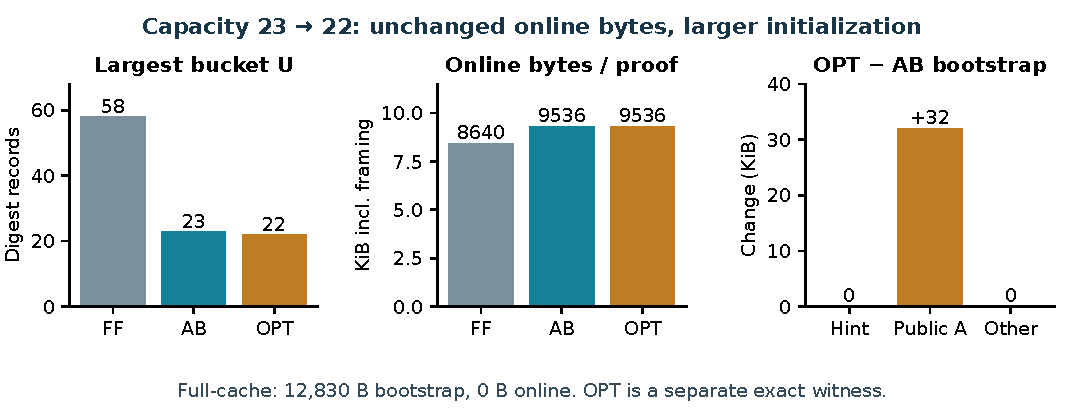
\includegraphics[width=\textwidth]{figures/fuel_layout_transfer.pdf}
\caption{Fuel capacity and cost under SimplePIR~\cite{simplepir}. AB is ours; other layouts are internal controls. Lowering $U$ from 23 to 22 retains 9536 online bytes and adds 32768 bootstrap bytes through expanded public $A$. Bars show deterministic counts; timing intervals appear in Table~\ref{tab:fuel-layout-transfer}.}
\label{fig:fuel-layout-transfer}
\end{figure*}

Independent reconstruction verifies all 2000 proofs (1500 PIR and 500 Full-cache) and 13760 recovered siblings against the pinned root and rejects corruption. The artifact retains paired schedules, traffic counters, parameters, bootstrap, and separate client/server RSS. These results concern the tested witness, without establishing efficient construction on larger instances.

\subsection{Certificate-record mirror}

The CT mirror contains 512 public log entries. Clients hash their known record and retrieve a proof against the experimental SMT commitment, not Google's CT root or certificate validity. Table~\ref{tab:ct_application_tcp} reports initialization and process memory; bootstrap transfers expanded public $A$ and hints without seed compression.

\begin{table*}[t]
\centering\small\setlength{\tabcolsep}{5pt}
\caption{CT mirror over loopback TCP using SimplePIR~\cite{simplepir}. AB is ours; other layouts are internal controls. Values are mean $\pm$ sample SD over five process pairs; timing uses process-pair means. E2E includes record hashing and root verification; bytes include application framing. Peak client/server RSS covers setup and transient allocations.}
\label{tab:ct_application_tcp}
\begin{tabular}{lrrrrrr}
\toprule
Method & Online (B) & E2E (ms) & Bootstrap (B) & Bootstrap (ms) & Client (MiB) & Server (MiB)\\
\midrule
First-fit & 17568 & $9.081\pm.253$ & 12279233 & $31.35\pm4.85$ & $42.55\pm.66$ & $51.60\pm.95$\\
AB & 20832 & $10.735\pm.907$ & 15392350 & $41.21\pm3.08$ & $51.15\pm.32$ & $81.51\pm2.03$\\
Nonempty-depth & 21344 & $11.330\pm.337$ & 14383745 & $36.49\pm8.73$ & $48.02\pm.60$ & $58.72\pm.73$\\
Full-cache & 0 & $.0254\pm.0059$ & 65566 & $1.118\pm.205$ & $6.22\pm.06$ & $4.35\pm.06$\\
\bottomrule
\end{tabular}
\end{table*}

All 2000 proofs (1500 PIR and 500 Full-cache) verify from 18476 recovered siblings. The paired Nonempty-depth/AB time ratio has 95\% interval $[0.929,1.196]$, without a stable advantage. First-fit is faster and sends fewer bytes; AB's bootstrap is 234.76 times Full-cache's. Unrestricted record retrieval makes Full-cache admissible: root authentication supplies integrity, not access control or database privacy.
